\documentclass[runningheads]{llncs}
\usepackage[T1]{fontenc}
\usepackage{graphicx}
\usepackage[super]{nth}
\usepackage{array}
\usepackage{hyperref}
\usepackage{xcolor}
\usepackage{colortbl}
\usepackage{booktabs}
\usepackage{hyperref,xcolor}
\hypersetup{
    colorlinks=true,
    linkcolor=[RGB]{18,10,143},
    anchorcolor=[RGB]{18,10,143},    
    urlcolor=[RGB]{204,78,0},
    citecolor=[RGB]{0,113,115}
}

\begin{document}

\title{Applying a Prompt Pattern Sequence for Decision-Making in Microservices Architectures}
\titlerunning{Prompt Pattern Sequence for Decision-Making in MSA}

\author{João José Maranhão Junior \inst{1}\orcidID{0009-0001-0049-4907} 
\and Jorge Melegati\inst{2}\orcidID{0000-0003-1303-4173}
\and Eduardo Guerra\inst{2}\orcidID{0000-0001-5555-3487}}
\authorrunning{Maranhão et al.}

\institute{Institute for Technological Research, São Paulo, Brazil, \email{jjunior@gmail.com},
\and Free University of Bozen-Bolzano, Bolzano, Italy, \email{jorge.melegati@unibz.it}, \email{eduardo.guerra@unibz.it}  }

\maketitle 

\begin{abstract}
Software architecture decisions are critical in a software project to ensure that systems meet functional and non-functional requirements. Microservice architectures have become popular in the industry, having a high amount of material available that was used in the training of large language models (LLMs). This paper explores the use of generative AI tools, such as ChatGPT, guided by a prompt pattern sequence to support architectural decision-making in microservices architectures. The proposed approach aims to provide structured guidance to software architects, helping them navigate in complex design challenges. To evaluate the prompt sequence, we conducted studies that revisited important architectural decisions made by large companies in the context of microservices architectures. Two industry case studies are presented: one involving the management of a large set of components in a financial institution, and the other focused on the front-end approach for a large-scale e-commerce platform in a pharmaceutical chain. The results demonstrate how five distinct prompt patterns deliver actionable insights tailored to each project’s unique technical and business constraints, enabling more informed decision-making. Retrospective feedback from architects highlights the effectiveness of the proposed prompt pattern sequence, which proposed solutions aligned to what was actually implemented. The findings suggest that generative AI, guided by well-structured prompt patterns, can support the decision-making process in microservice architectures.

\keywords{Prompt Patterns \and Software Architecture \and Generative AI \and Microservices}

\end{abstract}

\section{Introduction}

In recent years, rapid advancements in software engineering practices have led to the widespread adoption of microservices architectures, particularly in large-scale, complex systems. Microservices is an architectural approach in which an application is composed of loosely coupled and independently deployable services \cite{newman2015building,microservices2023}. Each service focuses on a specific business capability and can be developed, deployed, and scaled independently\cite{microservices2022}. While this architectural style offers benefits such as modularity, scalability, and fault isolation, it also presents significant challenges in both design and implementation \cite{fowler2014}.

A microservices architecture is a distributed software system architecture that comprises highly cohesive but loosely coupled services \cite{dragoni2017microservices}. A key challenge in this architecture is defining the boundaries of each microservice, which is essential to ensuring that the system remains with a good performance, fault-tolerant, and scalable \cite{balalaie2016microservices}. Poorly designed microservices can lead to a high number of dependencies between services, lack of fault tolerance, and overlapping responsibilities, ultimately degrading system performance \cite{richardson2018pattern}. Defining microservice boundaries requires a deep understanding of the system and domain knowledge, a process that is often iterative and error-prone. This task is typically performed by software architects and domain experts, whose skills and understanding of customer needs strongly influence the quality of the resulting architecture \cite{evans2003domain}.

The complexity of microservice design has led to the exploration of new technologies to aid the process. One such technology is generative AI, with GPT models having recently emerged as a valuable resource in software development. Generative AI has demonstrated capabilities in various software engineering tasks, including code generation\cite{liu2023improving}, testing, refactoring, and software design \cite{jiang2021survey}. Studies have shown that generative AI can aid in requirements analysis\cite{white2024chatgpt}, domain concept identification, and the generation of design artifacts such as class and sequence diagrams. In the context of microservices, the potential of generative AI and similar large language models lies in their ability to identify microservices\cite{stojanovic2023application}, analyze requirements, and provide design recommendations that align with system needs and architectural best practices \cite{meyer2023}. The large amount of material related to microservices architecture available that was consumed in the training of large language models (LLMs) creates a huge potential for its usage to support decision-making.

Due to the difficulties in obtaining the information using the conversational interface from tools based on LLMs, such as ChatGPT, a discipline named prompt engineering emerged \cite{Phoenix2024}. Prompt engineering can be defined as the process of structuring an instruction that can be interpreted and understood by a generative AI model. In this context, the prompt patterns \cite{white2023prompt} propose recurrent solutions that can be used in this interaction. For instance, some specific prompt patterns were proposed in the context of code quality improvement, refactoring, requirements elicitation, and software design \cite{white2024chatgpt}.

This paper proposes a prompt pattern sequence to support software architects in making critical architectural decisions based on the project's technical premises, quality attributes, uncertainties, and project context. Through this sequence, composed of five prompt patterns that guide interactions with ChatGPT, we aim to provide insights into how architects perceive this new interaction in decision-making in microservice architectures \cite{ayas2021,zdun2018}. This work evaluated the prompt pattern sequence in two industry use cases, revisiting past architectural decisions: one regarding a solution for managing a large number of software components and the other regarding a change in the front-end approach. The software architects involved in these decisions participated in an interview evaluating the prompt results and the approach itself. As a result, both architects evaluated that the obtained answers would be useful in the decision-making, reporting that they were aligned with what was implemented in practice. On the other hand, they also pointed out the lack of detail in some cases and suggested a more iterative approach to be able to go deeper into them.

%\section{Background}
%This study proposes using generative AI, such as ChatGPT, to assist software architects by offering personalized recommendations and insights in architectural decision-making. Through the use of Prompt Patterns, the aim is to provide clear and consistent guidance to architects, addressing recurring challenges in microservices architectures.

\section{Prompt Patterns Sequence}\label{prompt-patterns-sequence}

This work proposes new prompt patterns and a prompt sequence to be applied using generative AI conversational interfaces for architectural decision-making. They were described in more detail in a pattern paper focused only on them\cite{maranhao2024}.  The new five prompt patterns were designed to leverage the GPT model for suggesting architecture solutions aligned with the architect's decision power, technical premises, requirement uncertainties, quality attributes, and project context.  The next paragraphs describe each proposed pattern.

\texttt{Software Architect Persona} describes in the prompt a specialized persona for software architects, defining what is their decision scope to prevent answers that suggest actions outside of what can be done. It guides AI-generated responses to reflect the specific roles, objectives, and constraints architects face in complex projects. The goal is to tailor responses to be technically precise and contextually relevant, helping architects make informed decisions based on their current responsibilities.

\texttt{Technical Premises} is a pattern that introduces prompts to validate the technical premises used in architectural decision-making. Given the potential for AI-generated "hallucinations" (misleading or incorrect responses)\cite{meyer2023}, this pattern ensures that the AI justifies its suggestions with a list of specific technical premises. It allows architects to critically evaluate the accuracy and reliability of the AI’s outputs.

\texttt{Uncertain Requirement Statement} suggests creating prompts that explicitly state in the prompt what the uncertainties related to the software architecture \cite{silva2024using}. It helps architects plan for potential risks and impacts associated with these uncertainties, ensuring that the architecture is flexible enough to accommodate future changes. By proactively managing uncertain requirements, architects can better align the system with long-term business needs and technological trends.

Finally, the pattern \texttt{Quality Attribute Question} creates prompts to assist architects in evaluating the trade-offs and balancing quality attributes, such as scalability, security, and performance. Through an interactive questioning process, the AI tool gathers information about the system’s functional and non-functional requirements, helping architects make balanced decisions that optimize the integration of these quality attributes in architectural design.

Finally, \texttt{Architectural Project Context} integrates key project constraints into the decision-making process, such as development time, team size, and budget. It ensures that architectural solutions are theoretically sound and practically feasible within the project's limitations. The pattern helps architects design architectures that align with the business and technical requirements while navigating these constraints.

These patterns can be applied independently or in combination. After interactively evaluating various sequences and combinations, we propose a prompt sequence based on these prompt patterns, as illustrated in Figure~\ref{fig:flowchart-sequence}. The process begins by defining the role and objectives of the architect. Then, it moves on to assess technical premises and ask for solutions to handle uncertainties and balance quality attributes. The process concludes by prompting about the restrictions of the project context.

\begin{figure}[!ht]
  \centering  
  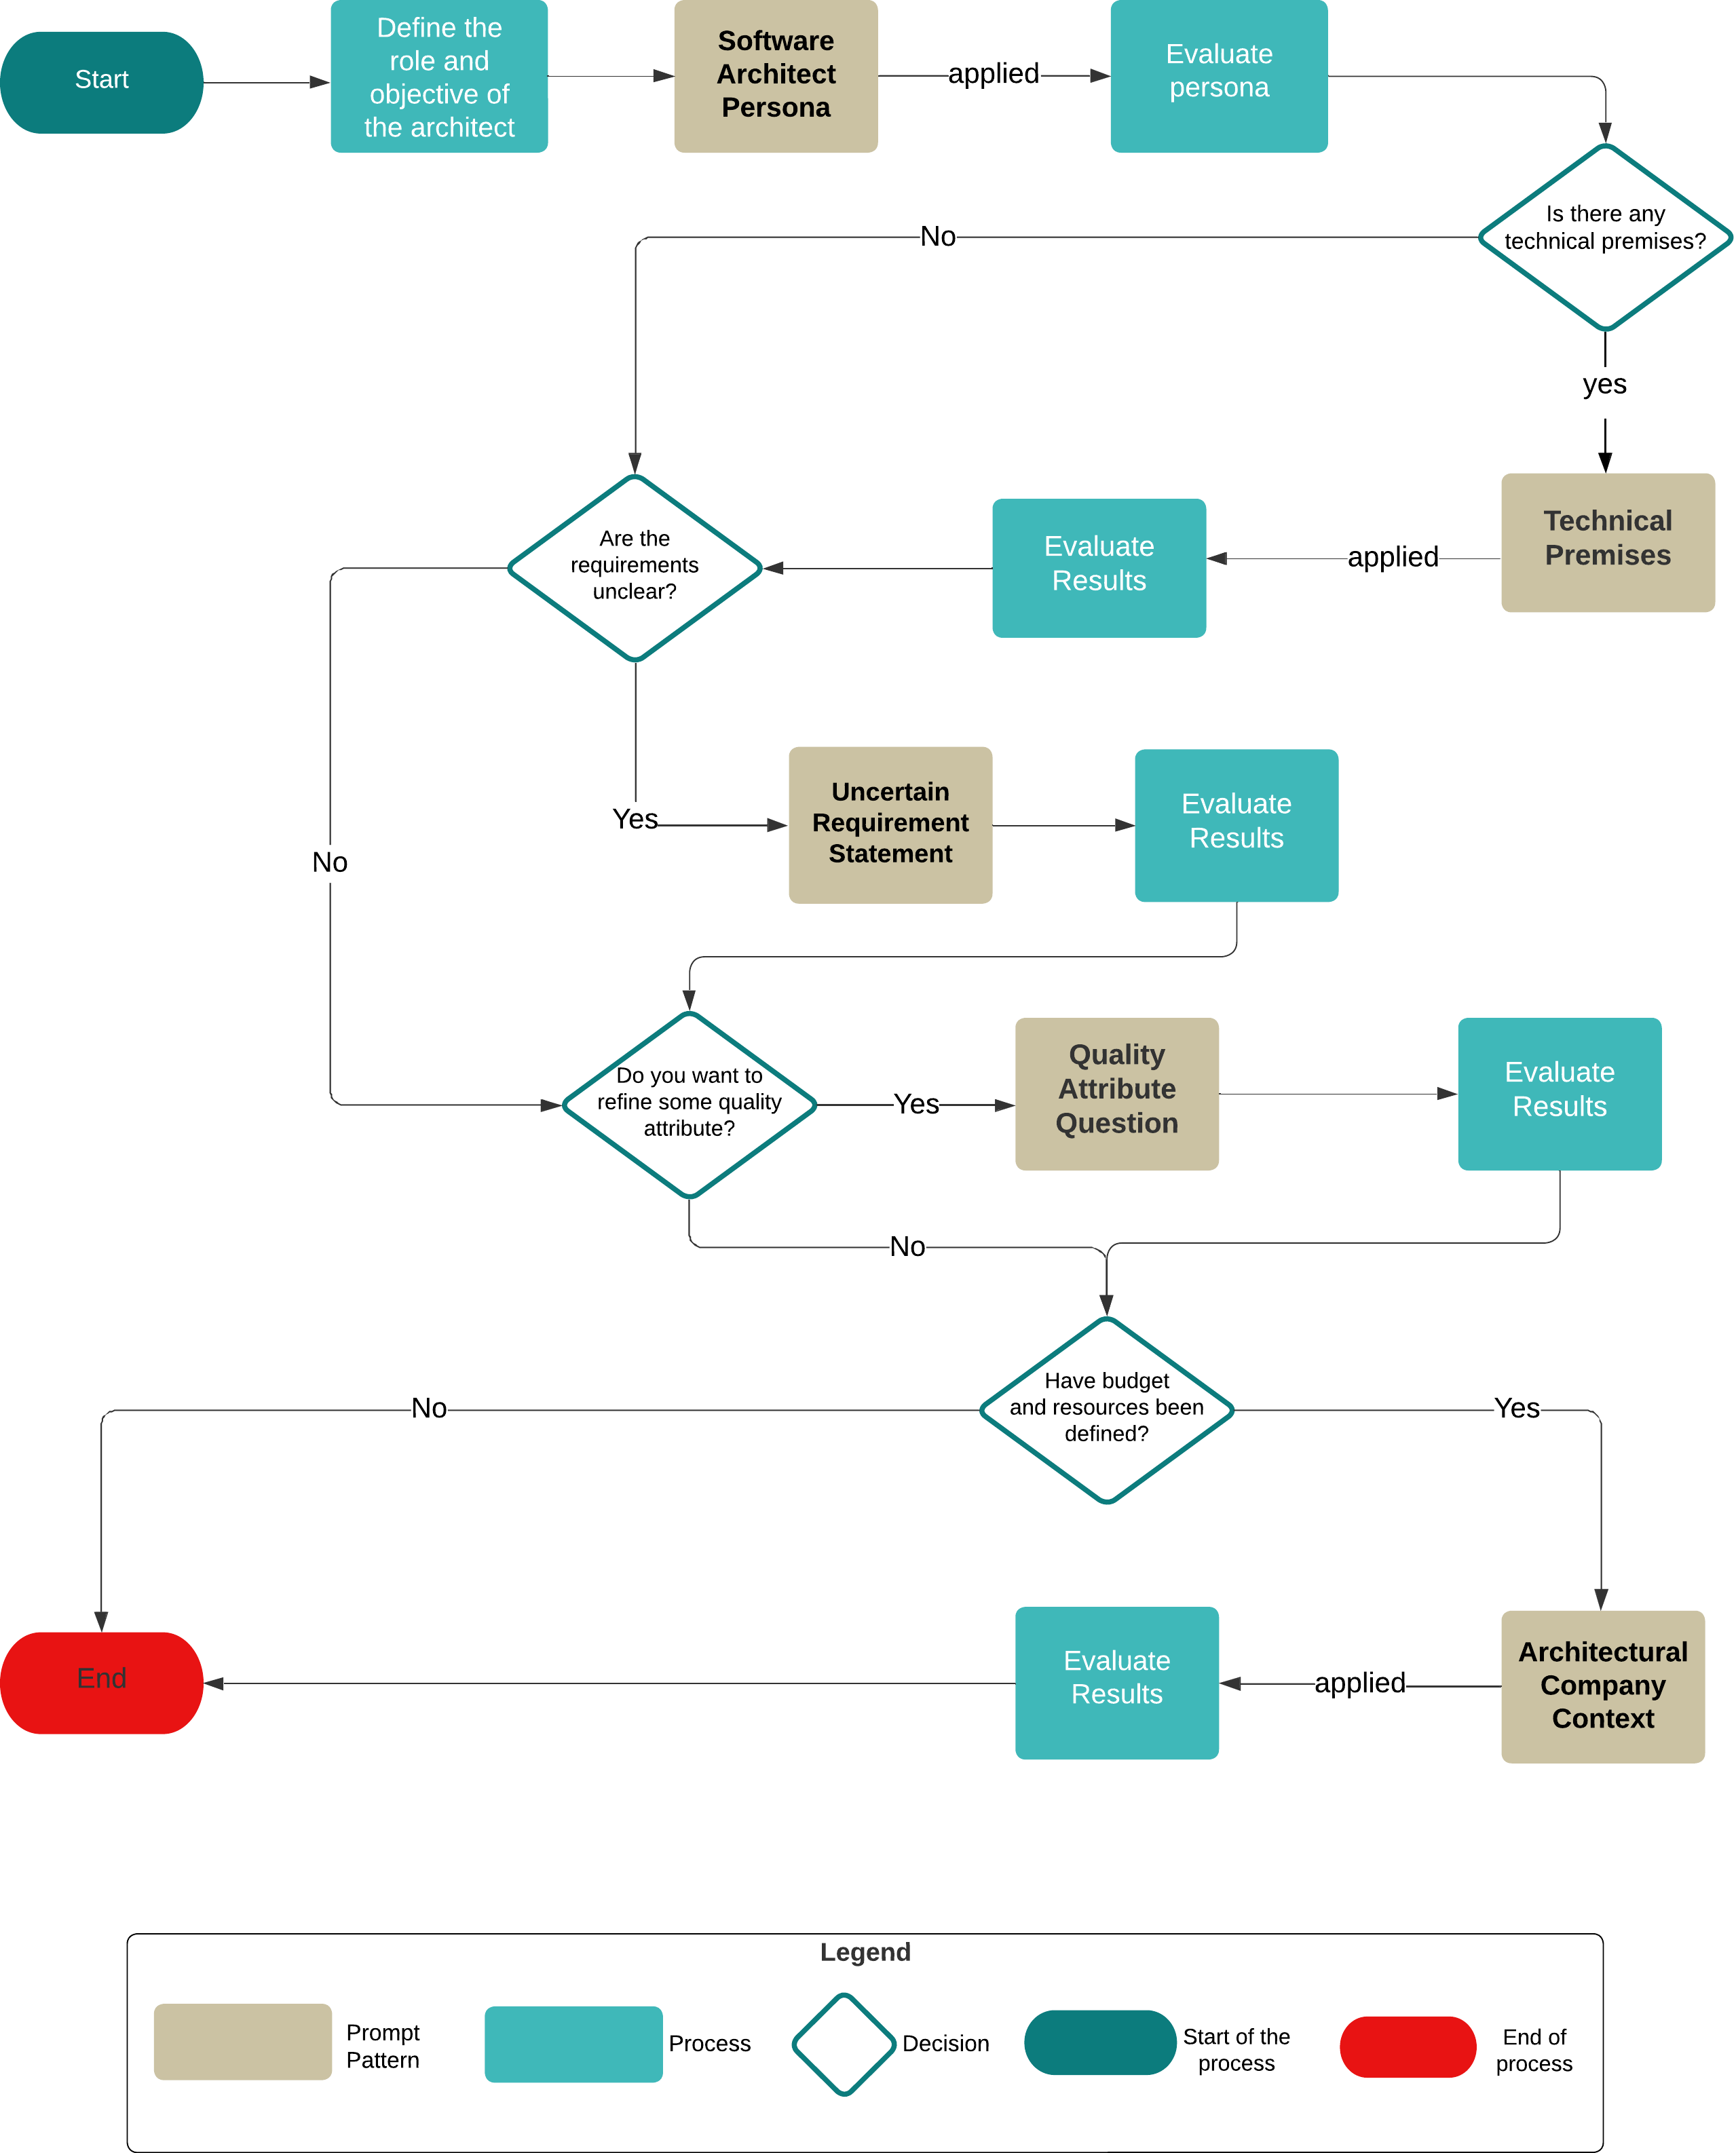
\includegraphics[width=0.95\linewidth]{flowchart-senquence.png}
  \caption{Decision Flow To Prompt Patterns Sequence}  
  \label{fig:flowchart-sequence}
\end{figure}

\section{Research Design}

The objective of this study is to evaluate whether the prompt pattern sequence proposed by this work can support the architectural decision-making processes, especially in scenarios involving microservices architectures. This study was guided by the following research question: \textit{What are the perceived benefits and challenges of using the proposed prompt sequence with generative AI tools in the decision-making in microservice architectures from the perspective of software architects?} 

To achieve that goal, we identified important architectural decisions made in real software projects to be used as the basis for this evaluation. Based on the project information collected, we recreated the existing scenario when the decision was made in the prompts and used the prompt pattern sequence to retrieve information from ChatGPT that could support the decision-making. After that, we interviewed a software architect who participated in the decision and followed the implementation of the solution, having information regarding its consequences and the challenges faced by the team. Based on that, we assessed the applicability of the proposed approach in supporting architectural decision-making.

The research method used in this study is inspired by characteristics of case studies\cite{runeson2012case} and retrospective studies ~\cite{desouza2005experiences}. From case studies, we considered observation of real scenarios to address relevant and realistic factors. Since architectural decisions usually involve complex specific attributes and relationships, using real cases allows the representation of the complexity of this process. Considering similarities with retrospective studies, we reviewed decisions and their consequences from completed projects, as performed by other studies~\cite{hayes2011impact}. However, in our case, we not only analyzed past decisions but simulated their context to evaluate the proposed technique. 

%The combination and minor modifications to established methodologies were not intended to introduce new features but were essential to address the particular nuances of our research question. This approach maintains the analytical nature of retrospective analysis and the observational strengths of case studies while providing the necessary structure to explore the specific influence of AI-generated data through the prompt pattern sequence on architectural decision-making.

\subsection{Research Steps}

The research methodology for this study was executed in the following five steps: (1) recruit companies to participate in the study, (2) select and document target design decision, (3) execute the prompt pattern sequence, (4) present the results and interview a software architect involved in the decision, and (5) perform a qualitative analysis of the prompts and interview answers. The study was conducted between October 2023 and March 2024, and GPT-4o was used to execute the prompts.

%\begin{figure}[!ht]
%    \centering
%    \caption{\centering Research Method Steps.}\label{research-method}
%    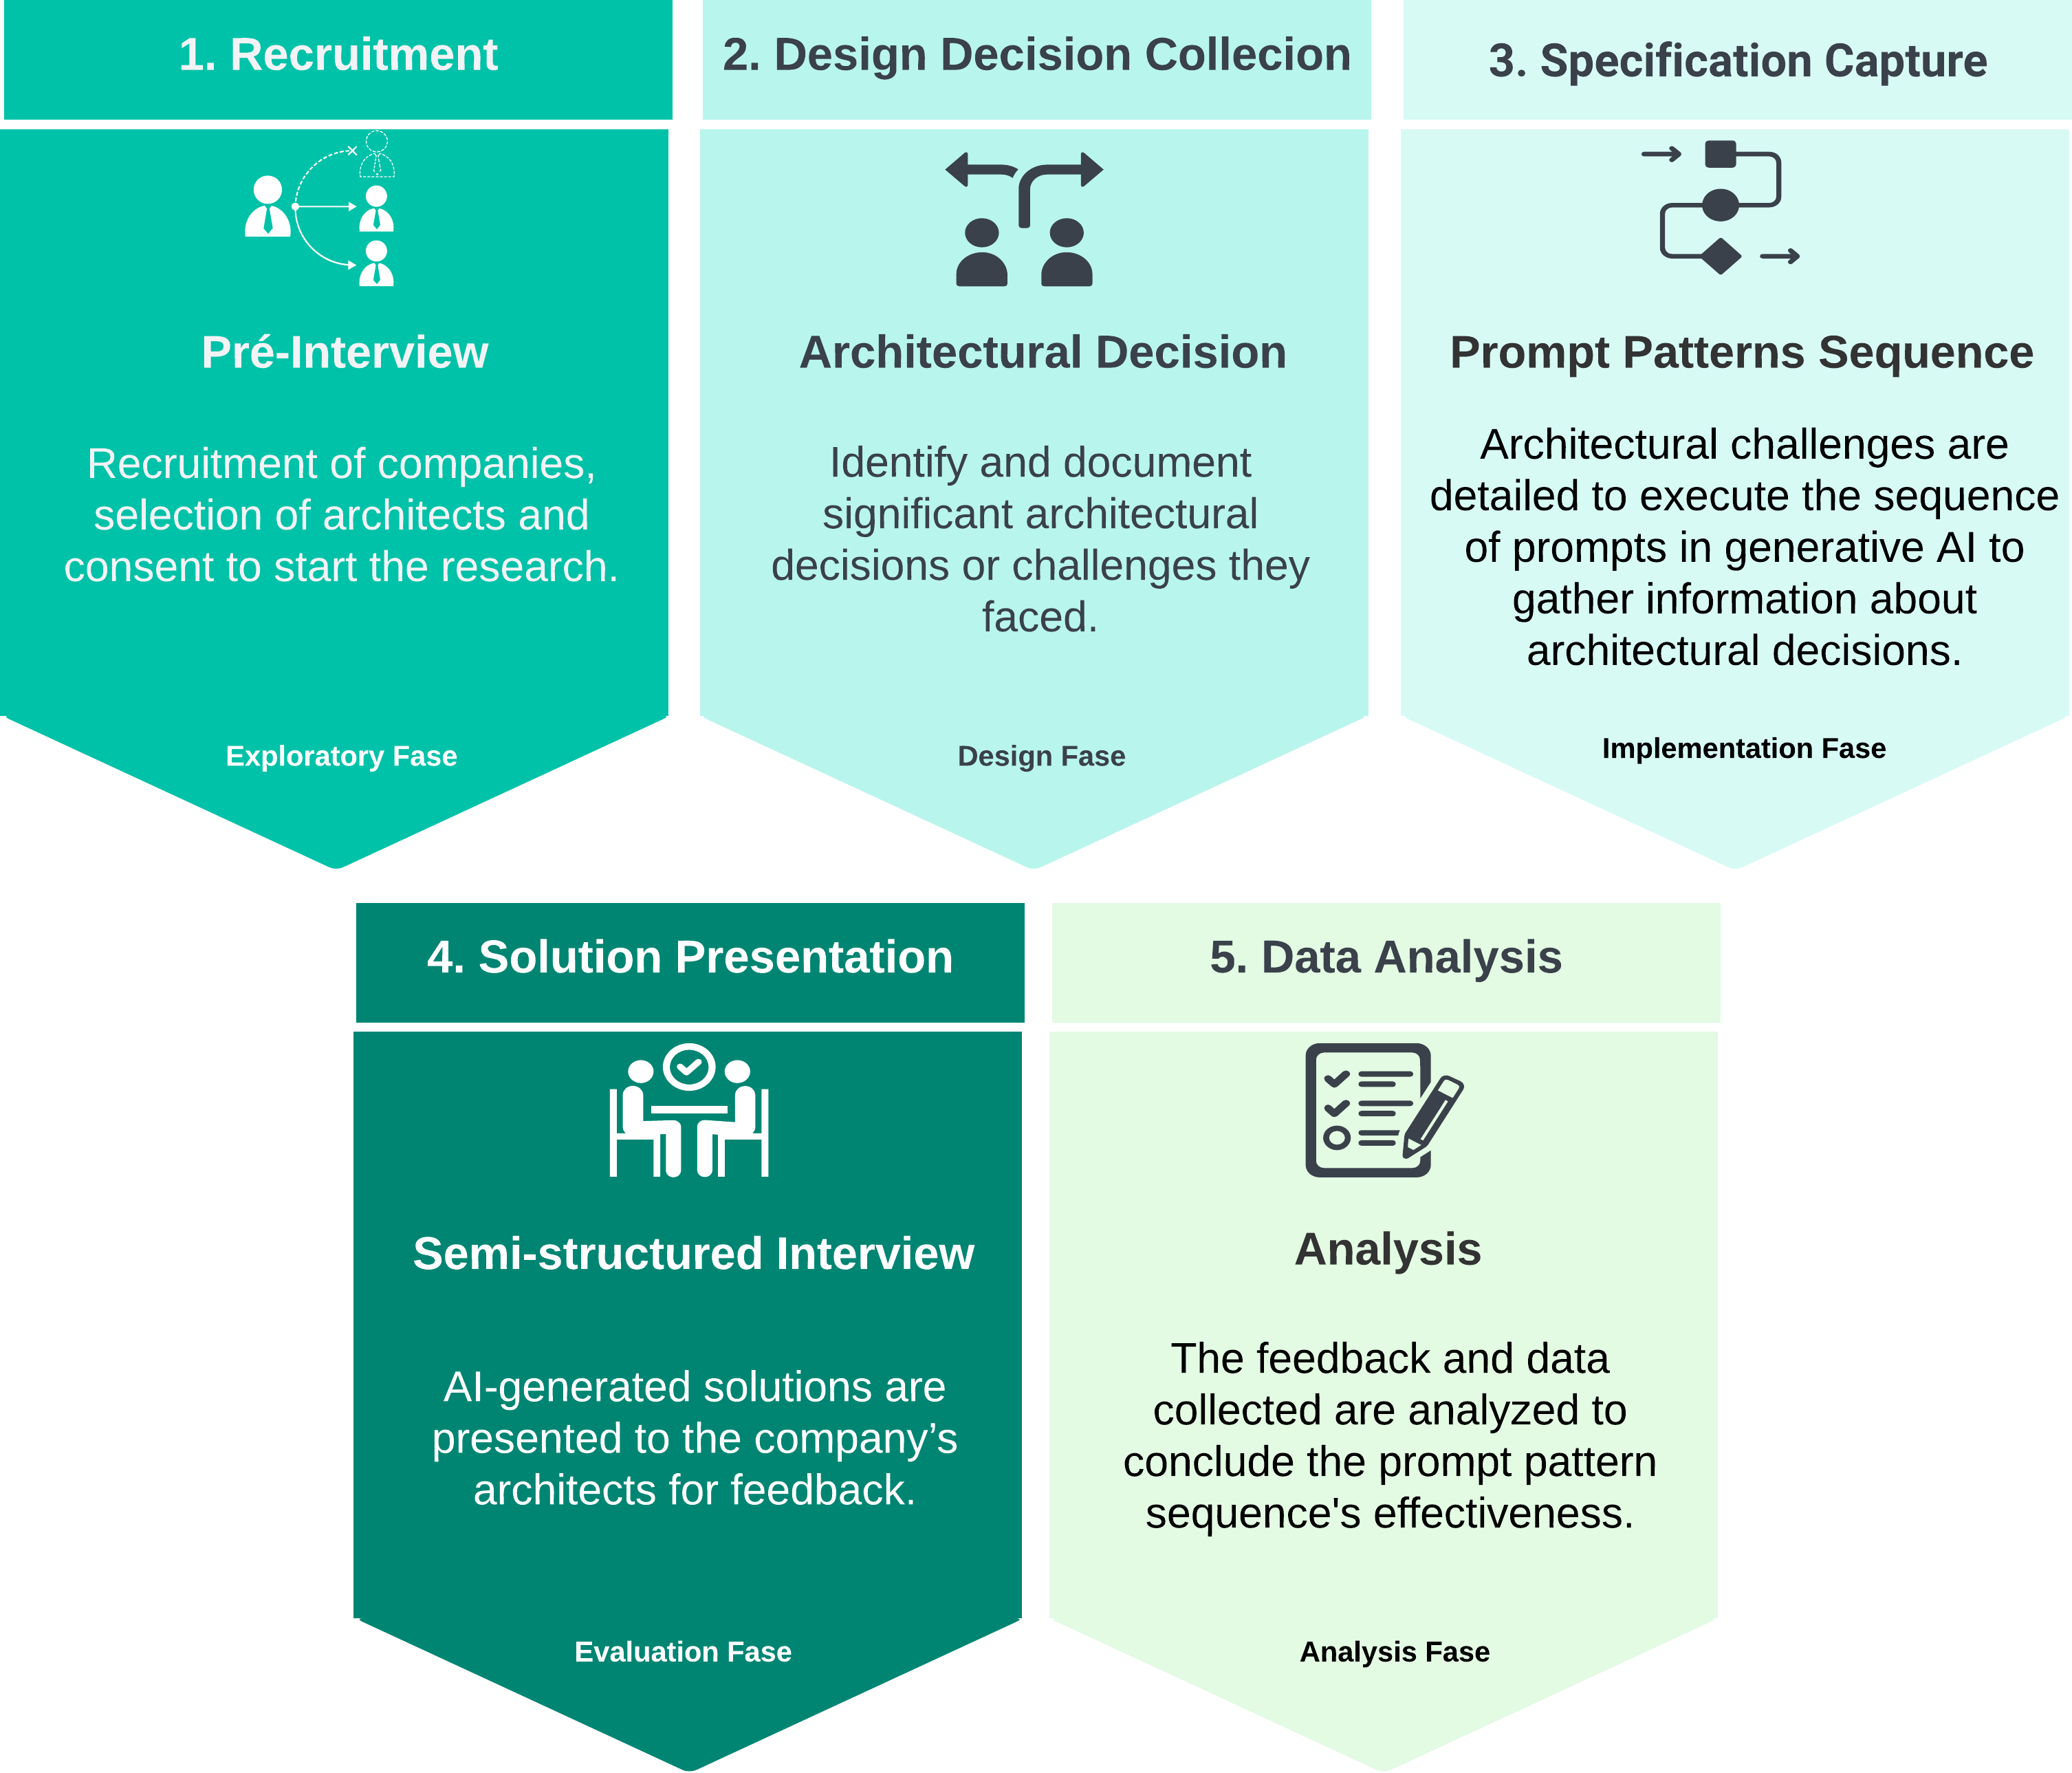
\includegraphics[width=0.94\textwidth]{research-method.png}    
%\end{figure}

For the recruitment phase, we considered that projects had to meet three inclusion criteria: (a) be a recently completed project to ensure up-to-date and relevant architectural practices; (b) it must involve significant architectural decisions related to microservices; (c) participating company should be willing to provide detailed project data, including technical specifications, decision-making processes, and results.

Recruiting such companies posed a challenge due to confidentiality concerns\cite{runeson2012case}. To address this, convenience sampling was used, focusing on companies with professionals inside the contact network of the researchers\cite{marshall1996sampling}. After the prerequisites and methods were presented, two Brazilian companies operating in the Brazilian market agreed to participate in the study. Company A (leader in car financing) and Company B (leader in pharmaceutical retail with more than 3000 stores) were selected. Both of them have systems with microservices architectures that face interesting technical challenges.

As the second step, a relevant design decision was selected for each project and analyzed through meetings with their architects. The goal was to select a specific architectural decision to focus and retrieve information to be used to create the prompts of the prompt pattern sequence. In the third step, the prompt patterns were used to create the prompts according to each company’s specific architectural scenario. The prompts were executed for each scenario and prepared to be presented to the software architects.

As the fourth step, the results of the prompt sequence were presented to the architects, and interviews were conducted following the protocol presented in the next subsection. The questions were focused on asking the architects to evaluate AI-generated responses based on the prompt pattern sequence and their usefulness in the retrospective scenarios. Questions about the architects’ expertise were also collected to understand their professional background, making sure they have the appropriate experience to judge the results. In the fifth step, we conducted a qualitative analysis focused on the architects' perceptions regarding the AI-generated responses, considering the challenges in the project and the developments that happened later. We also evaluated how they evaluated the prompt patterns and the respective prompt pattern sequence to extract relevant information from the AI tool.

% After completing the interviews, we will analyze the specific points of each prompt and the sequence of prompt patterns through two sources of information: the architect's perception of the analyzed scenario and the information generated by the prompt patterns. This analysis aims to identify the most effective prompt patterns that captured respondents' interest and provide insights into the specific elements or characteristics that contributed to this perception. 


% These interviews were recorded using the interview protocol described in Table~\ref{table:methodology} with~IQ, and each part (\textbf{Interview Introduction}, \textbf{Software Architect Profile}, \textbf{Prompt Patterns}, and \textbf{Prompt Pattern Sequence}) of the interview is explained below. The architects were asked about the usefulness of the responses generated by AI in the scenarios in which they participated so that they could retrospectively evaluate the AI's suggestions through the sequence of prompt patterns.



\subsection{Interview Protocol}

The interview started with a comprehensive introduction in which the participants are reminded of the consent terms to ensure their complete understanding and agreement. Following this, a clear explanation of the research objectives was provided to help participants understand the study's aims. The research protocol was also outlined, giving participants a clear understanding of the procedures and expectations during the study. Finally, participants were asked permission to record the sessions for further analysis.

As the first interview section, participants are asked detailed questions to gather background information and assess their expertise in software architecture. They are first asked about their experience working with software architecture, followed by a request to describe their professional trajectory and main experiences in software architecture. Participants are also asked about the duration of their employment at their current or previous companies (Company A or B) and the roles they have performed there, which provides context on their responsibilities and influence on decision-making processes within the company.

Further, the interview moves to the prompt patterns section, where we seek to gain insight into the perspective of architects regarding the architectural recommendations generated by AI using prompt patterns created in this work. The questions presented in Table 1 were used to guide the interview, which followed a semi-structured format. For each prompt pattern, the pattern was explained and the prompt and the respective answer presented. The architect then answer the questions regarding that pattern. In the end, the questions regarding the pattern sequence were asked. 

\begin{table}[!ht]    
    \centering
    \caption{Questions about the prompt patterns and prompt patterns sequence.}
    \label{table:methodology}
    \begin{tabular}{p{4.8in}} 
        \toprule
        \hline                 
        \textbf{Prompt Pattern Questions} ~\\ \hline        
        \textit{Would the information generated by the prompt have been useful at the time of the project?}
        
        \noindent\textit{Which of the responses generated coincides with what was implemented?}
        
        \noindent\textit{Is there any information in the generated responses that you disagree with?}
        
        \noindent\textit{Is there information you agree with in the generated responses that you would implement?}
        
        %\noindent Questions about the usefulness of architectural suggestions generated by prompt patterns are answered by retrospectively analyzing the project to capture the software architect's insights. ~\\ 
        \midrule        
        \textbf{Prompt Patterns Sequence Questions} ~\\ \hline
         % \rowcolor{gray!19} \textbf{Prompt Sequence Questions}   ~\\ \hline
        \textit{What do you think of the proposed sequence?}
        
        \noindent\textit{Does this sequence fulfill the objective of supporting architectural decision-making?}
        
        \noindent\textit{Were any steps unnecessary and could be removed?}
        
        \noindent\textit{Are there any steps that need to be added?}
        
        \noindent\textit{Would you make any changes to the sequence of prompts applied?}
        %&\noindent Questions regarding the usefulness of the sequence used for prompt patterns.~\\ 
        \hline
        \bottomrule
    \end{tabular}    
\end{table}

For each pattern, we started asking the participants a fundamental question: whether AI-generated information would have been helpful during the project to evaluate the practical applicability of prompt patterns. Further, the participants were requested to elaborate if the responses were aligned with what was implemented and discuss any discrepancies or agreements with the AI suggestions.

Following that, the sequence of prompt patterns was assessed. Participants were asked for their thoughts on the proposed sequence and whether it meets the objective of supporting architectural decision-making. They were encouraged not just to criticize but also to suggest if any steps are unnecessary or if any additional steps could be added to enhance the process. 

\section{Industrial Case Studies Description}

This section reports the results of applying the prompt pattern sequence in the context of projects from two companies, a financial institution, and a pharmaceutical company, that will be referred respectively to as COMPANY A and COMPANY B. The focus is on evaluating the perceived benefits and difficulties of applying prompt pattern sequences through generative AI to assist in the architectural decision-making process from the perspective of software architects. In the description of each case, a link to the execution of the prompts is provided, and all names used in the prompts are fictitious for confidentiality reasons. 

In both cases, the software architect who participated in the interview had experience in microservices architectures and had appropriate knowledge to judge the answers. They also participated in the decision process targeted by the study, following the implementation of the solution and the developments that followed it. Based on that, we judged their experience appropriate to evaluate the result of the prompt sequences. 

%\subsection{Study Goals}

%In Chapter~\ref{prompt-patterns-sequence} of this research, we have developed a sequence of five new prompt patterns for software architects. These patterns were created in a hypothetical scenario for a CRM project at a startup. The purpose of this research was to incorporate the perspective of software architects into a real-world project, as we addressed \textbf{\textit{RQ\textsubscript{3}}}. To determine the effectiveness of the pattern-based prompt sequence applied in Section~\ref{prompt-patterns-sequence}, we need to analyze its ability to support architects' decision-making process, its suitability and ease of implementation, and its advantages and disadvantages. Our primary focus is on answering the following research question:

%What are the perceived benefits and challenges of using the proposed prompt sequence with generative AI tools in the architectural decision-making process from the perspective of software architects?---\textit{This includes the opinions of software architects on real projects about the usefulness of generative AI information through prompt patterns sequence and its potential to streamline the decision-making process in their organizations.}

%Each study was a collaborative effort, utilizing two different architectural decisions and applying the same sequence of prompt patterns written in English to analyze the responses. The initial stage involves identification and an overview of the system to identify the architectural decision. In the subsequent step, the sequence of prompt patterns is applied to provide information to assist in decision-making, followed by the contribution of software architects to evaluate the information from the prompt sequence. The main techniques used for data collection were semi-structured interviews carried out in Portuguese and freely translated into English, and open analysis procedures were used to analyze the data based on immediate results.

%This study uses a combination of case studies and retrospective methods, slightly adapted to meet our specific research objectives, this study uses a combination of case studies and retrospective methods~\cite{desouza2005experiences,runeson2012case}. Case studies observe and document architectural decisions in real-world scenarios~\cite{gustafsson2017single}, while retrospective studies review completed projects to assess whether generative AI suggestions could have influenced past decisions~\cite{hayes2011impact}. 

%The goal is to evaluate how the Prompt Patterns Sequence impacts decision-making by comparing the decisions made during the project to the information generated through the sequence. By simulating decision points with new AI-based inputs, we assess the potential impact of AI on architectural decisions.


\subsection{Financial Institution - COMPANY A}

COMPANY A\footnote{Full prompt: \url{https://chat.openai.com/share/5604c457-13b2-4213-90da-8b59838673fc}} has a system that adopts a microservices architecture and manages over 18,000 software components using various technologies and frameworks. 
%It relies on CI/CD processes facilitated by Jenkins, Spinnaker, and UrbanCode, with SonarQube for quality testing and Veracode for security. 
The scenario chosen to be analyzed concerns COMPANY A's change management process, which is critical in this type of architecture. The software versions could not be released if code coverage fell below a threshold or had critical security issues, and the fact that analysts manually gathered quality and security metrics caused delays and increased risks. The focus of this study was on the architectural decision regarding how to implement an automated solution to centralize and streamline the change management process by integrating several key technologies. 

%With six years of experience in software engineering and three in software architecture, Architect A advocates for developers to understand architecture. He is also actively involved in the academic community, particularly with tools like GitHub Copilot and ChatGPT, recognizing the importance of correctly applying design patterns to solve common system issues.

For the first prompt pattern, \texttt{Software Architect Persona}, Architect A emphasized the significance of defining a specific persona to enable the AI to tailor its responses more effectively to their needs. This approach made the interaction more relevant and practical. Architect A also confirmed that this pattern helped to narrow the scope of the AI's responses, ensuring that the information generated aligned with the project’s architectural requirements. 

Architect A appreciated the detailed technical context in the second prompt pattern, \texttt{Technical Premises}, noting its reflection on practical project considerations. He emphasized the importance of technical assumptions in checking the validity of AI-generated solutions to specific technologies. Architect A highlighted the effectiveness of the prompts in the guidance present in the answers. He believed that it could help the team to implement solutions, such as a dashboard using Angularand TypeScript, ensuring alignment with the project's architecture and security practices.

He also noted that the prompts could have addressed resilience-related issues by suggesting appropriate delays for report availability. Architect A shared an example: \textit{"When we integrated with a tool like Veracode, a report with security information was generated, but we didn’t realize it wasn’t available instantly. This led to a problem when we checked the report prematurely."} He explained that a delayed query job could have resolved the issue and that using this approach earlier would have saved time. The prompts could have proactively guided the team in implementing such resilience measures.

% The third pattern \texttt{Uncertain Requirement Statement} highlighted the challenge of developing and maintaining integrations without predefined API contracts. Architect A noted that while adopting an API management tool can help, it's not always feasible, particularly with market products like Veracode and Sonar, which offer limited customization. Architect A suggested implementing contract tests in the pipeline, which is especially useful. Such tests would verify the integration during updates, allowing issues to be caught early rather than waiting for user feedback. However, due to tight deadlines, this strategy was not implemented, though Architect A believed it could have mitigated issues, even if not solving them entirely. Architect A further explained that the team had to accept certain risks when integrating without a defined contract, recognizing the potential security vulnerabilities and their impact on software evolution and maintenance. He also commented on the strategy and planning suggestions, noting that some seemed overly standardized, such as the recommendation to adopt an API management tool.

The answer to the third pattern \texttt{Unclear Requirement Statement} suggested developing API contract integrations for consuming microservice APIs using contract-first and testing them in the CI/CD pipeline. Architect A noted that while adopting an API management tool can help, it is not always feasible, especially with off-the-shelf products like Veracode and Sonar that offer limited customization. However, due to tight deadlines, this strategy was not implemented, although Architect A believed it could have mitigated the issues at the time, even if it did not completely solve them.

Architect A found that the prompt stimulated the generative AI to ask insightful questions when using the fourth \texttt{Quality Attribute Questions} pattern to ask about scalability and resilience. According to him, the considerations about quality attributes generated by the prompt pattern demonstrated its ability to highlight critical aspects of system design that may not be immediately obvious, helping architects build more robust systems. All necessary points were addressed, and as more information was provided, the AI developed a more detailed solution, proposing improvements for performance, quality, and scalability. Architect A found it particularly valuable that the AI suggested additional solutions, such as implementing caching mechanisms, increasing horizontal and vertical scalability, and delegating certain functionality to other system components. These efforts went beyond what was initially requested. The extra attention to detail and proactive suggestions were greatly appreciated and exceeded the architect’s expectations.

When prompting about the \texttt{Architectural Project Context}, ChatGPT underestimated the implementation timeline compared to what was actually needed. Even though Architect A appreciated aligning the AI's suggestions with effective software architecture practices. The suggestions provided a vision consistent with the project's architectural goals, even if the timeline required adaptation.

Architect A confirmed that the \texttt{Prompt Patterns Sequence} would be helpful for architectural decision-making in the described scenario. The detailed guidance provided by the AI aligned well with the project's needs, and its recommendations closely matched what was implemented in practice. While no steps were considered unnecessary, Architect A suggested making some parts more concise and adding an interactive element for exploring specific topics further.

Architect A emphasized that the sequence effectively supported architectural decision-making, particularly in areas like resilience and quality. It would have been extremely useful during the project's development, potentially facilitating faster delivery of high-quality solutions. The prompts' structured and detailed approach provided valuable and relevant guidance that aligned well with the project's practical needs. While no steps were unnecessary, Architect A reiterated the benefit of adding an interactive feature for deeper exploration of specific topics if needed. The following quote represents Architect A assessment: \textit{"I wouldn't change the chat prompts significantly. The sequence was engaging and made sense. Some minor modifications might be needed to adapt to specific needs, but the accuracy of the chat's recommendations, which closely resembled what we applied in practice, was impressive."}

\subsection{Pharmacy Chain - COMPANY B}

COMPANY B\footnote{Full prompt: \url{https://chat.openai.com/share/775a0eae-b826-4ab3-95ac-eca4f60bf649}}, one of the Brazilian largest pharmacy retail chains, is overhauling its customer service interface across 3,000 stores to improve efficiency and modernize interactions. Each store’s system handles tasks like price checks, order processing, and compliance with Brazil’s LGPD, emphasizing the need for a robust solution. The problem that was chosen to be targeted was the inefficiency of the front-end approach, which was leading to potential customer dissatisfaction and maintenance issues. The pharmacy chain needed a scalable, user-friendly, and highly available front-end system to handle operations, including 24/7 locations, with minimal disruptions. The project team had to decide on a new architectural approach for the front-end system. 

Architect B emphasized the importance of defining the \texttt{Software Architect Persona} to guide project decisions and confirmed that it should be the first prompt in the sequence. Regarding \texttt{Technical Premises}, Architect B agreed that the prompt’s suggestion for the adoption of micro front-ends\cite{microservices2022} aligned with the project’s technical requirements and praised the detailed comparison of architectural approaches. He confirmed that the architectural decision generated by the prompt patterns was the same decision made in the project, as stated in the following: \textit{“We reached the same conclusion: that micro front-ends, given the scalability and multidisciplinary team, would fit the product.”} He also appreciated the presentation of the advantages and benefits of each architectural approach, which provided a solid basis for comparison. Even though the suggestion was agreed upon, the architect missed a question about the current backend configuration before recommending the usage of micro front-ends. 

The pattern \texttt{Uncertain Requirement Statement} addressed technical variations, network reliability, system integration, and user adoption uncertainties. Architect B acknowledged the importance of having more intuitive interfaces and noted that 90\% of the system screens were redesigned in that direction, as suggested by the prompt. He also appreciated the recommendation to consider technologies such as GraphQL or BFF, which aligned with the project’s modernization efforts. As a critic of the answers received, the architect expected more specific and technical recommendations, such as including Kubernetes for management and scaling.

The \texttt{Quality Attribute Question} addressed quality attributes such as usability, scalability, and testability. The participant expressed satisfaction with how the prompt clarified doubts and decision-making based on the specified quality attributes. He found the suggestions helpful for generating features to collect user feedback. Architect B remarked: \textit{"It’s nice to have continuous evolution and faster feedback... I thought it was cool; it’s something we don’t have today."} As in the other questions, Architect B missed more details in the answers, this time in the testing recommendations. He mentioned that the discussion could include more details on the types of tests that would be most effective, such as integration or unit tests. 

The prompt for the \texttt{Architectural Project Context} focused mainly on the team organization and the delivery strategy. Architect B valued the insights related to the team structure and sprint cycles. He also appreciated the recommendation for using the micro front-ends to improve component scalability. On the negative side, Architect B expressed concern about potential bias in the cloud vendor recommendations, specifically the exclusion of Google Cloud Platform (GCP) in favor of AWS and Azure. He suggested that the prompt should take a more neutral stance toward specific vendors.

Evaluating the prompt sequence, Architect B confirmed that the \texttt{Prompt Pattern Sequence} effectively would support architectural decision-making in the evaluated context, particularly regarding resilience and quality. The sequence offered valuable guidance, leading to suitable solutions quickly, highlighting that the AI’s recommendations were closely aligned with the solutions implemented in practice. Architect B suggested reorganizing the sequence, bringing the Quality Attribute Question pattern closer to Technical Premises, as he felt that non-functional requirements are closely related to technical assumptions. He also recommended adding an interactive element, allowing for additional specific questions to explore topics more deeply.

\section{Discussion}

Integrating generative AI tools into the architectural decision-making process by using the proposed prompt pattern sequence has demonstrated substantial benefits and has surfaced areas for improvement, as noted by software architects. This discussion delves into these aspects, emphasizing the value of prompt patterns and their sequence in enhancing architectural decision-making.

From their professional perspective, software architects identified numerous advantages in using sequence prompt patterns with generative AI tools. A key benefit is the structured guidance that prompt patterns offer, allowing architects to address various architectural questions systematically. The AI’s ability to generate relevant, context-specific information boosts the efficiency of the decision-making process. Furthermore, the prompts’ focus on critical factors such as resilience, scalability, and technical premises ensures that essential architectural considerations are not overlooked.

However, using generative AI also poses challenges. Architects observed that the AI sometimes generates generic or overly broad recommendations that need more specificity for complex technical environments. Additionally, there is a need for more iterative and detailed follow-up questions to explore issues further, which the current prompt patterns may need to address fully. This lack of interaction can also be due to the sequence adopted in the study, in which the prompts were generated before the interview. In a real setting, the software architects do not need to be restricted only to these patterns and strictly follow the proposed sequence. By using it as a guide, it is possible to explore some of the answers in more detail with some additional prompts.

According to the participants, the information generated by the prompt patterns would have been beneficial during past projects. For example, prompts for patterns like \texttt{Technical Premises}, \texttt{Quality Attribute Question}, and \texttt{Uncertain Requirement Statement} could have provided more precise direction for architectural decisions, potentially preventing integration and performance issues. The structured approach to identifying and addressing uncertainties would have been valuable in mitigating potential risks.

AI-generated responses also aligned with actual implementations in the two industry case studies. For instance, the micro front-end solution recommended as answers to the \texttt{Technical Premises} and \texttt{Uncertain Requirement Statement} prompts in the pharmacy chain project was adopted. This enabled independent development and scaling of features across multiple stores. Similarly, strategies implemented in the project mirrored the AI’s emphasis on cloud-based solutions for scalability and resilience to microservices.

In both studies, architects also noted divergences between AI-generated responses and their specific needs, particularly regarding the generality of particular recommendations. In the case of the financial institution, suggestions for API management and integration approaches sometimes needed to be more abstract or fully aligned with the project context, as reflected in prompts like \texttt{Uncertain Requirement Statement} and \texttt{Architectural Project Context}. In the pharmacy case, some recommendations to address uncertainties were general and, according to Architect B, needed to be more specific.

Controversial points in the AI’s output also emerged. In the financial institution case, disagreements arose concerning project delivery deadlines, highlighting a potential limitation in the AI’s understanding of complex project timelines regarding using the \texttt{Architectural Project Context} pattern. Similarly, in the pharmacy scenario, the AI’s recommendation of a specific cloud vendor, while omitting others, raised concerns about its ability to provide comprehensive, unbiased information.

Despite these challenges, architects agreed on several AI-generated suggestions they would implement. In the case of financial institutions, AI recommended more robust contract testing to ensure API consistency and a message broker approach to maintain loose coupling and guarantee message delivery. These recommendations were noted in the \texttt{Technical Premises} and \texttt{Uncertain Requirement Statement} prompts patterns. In the pharmacy case, the AI’s suggestion to include a "suggestions and improvements" feature in the front end to enhance quality attributes was appreciated, as reflected in the \texttt{Quality Attribute Question} prompt pattern.

Architects responded positively to the sequence of prompt patterns, praising its logical flow and comprehensive coverage of critical architectural considerations. The sequence effectively guides architects through a structured decision-making process, ensuring that all critical aspects are addressed thoroughly. Overall, they judged that the sequence supports architectural decision-making by providing a clear structure for evaluating and resolving architectural challenges, ensuring decisions are well-informed and aligned with project requirements.

While architects did not identify any unnecessary steps in the sequence, they suggested that some prompts could be more concise and focused on avoiding redundancy, streamlining the decision-making process, and increasing their effectiveness. Additionally, they recommended adding more interactions, allowing the architect to ask follow-up questions to explore specific topics in greater depth. While this lack of interaction was also due to the structure of the study, as stated previously, we agree that the sequence could have this aspect more explicitly represented. One architect proposed reorganizing the sequence, suggesting that quality attribute-related issues be addressed earlier, closer to the \texttt{Technical Premises} prompt. This change was argued to improve accuracy, as non-functional requirements are closely tied to technical assumptions.

An important point to be highlighted is that the decisions targeted in this study were in the context of microservice architecture, which is a popular architectural style in the industry with plenty of material available. That has an influence on the material used for training the generative AI, which also contributes to the correctness and precision of the answers. Because of that, the results of this study should be considered in the context of this specific architectural style. 

%The sequence of prompt patterns proposal with generative AI tools significantly benefits architectural decision-making by offering detailed, systematic, and relevant information. While there are areas for improvement, the overall approach enhances the robustness and reliability of architectural decisions, ensuring they are better aligned with project objectives and requirements.

\section{Conclusion}

The adoption of generative AI tools, guided by the proposed prompt pattern sequence, has demonstrated potential in supporting architectural decision-making for microservices architectures. 
This study applied the sequence in two real-world scenarios, in a financial institution and in a pharmaceutical company, highlighting how AI-generated insights, structured through prompt patterns, can enhance decision-making by providing architects with relevant, context-specific guidance. According to the participants, the five proposed prompt patterns, namely \texttt{Software Architect Persona}, \texttt{Technical Premises}, \texttt{Uncertain Requirement Statement}, \texttt{Quality Attribute Question}, and \texttt{Architectural Project Context}, provided a systematic approach in the usage of generative AI tools to address critical architectural challenges while ensuring that technical and business constraints were considered.

Architects who participated in the study provided valuable feedback on the sequence, underscoring its practical relevance. They particularly highlighted its effectiveness in ensuring that critical considerations like scalability, resilience, and quality attributes were not overlooked. The study also identified areas for improvement, such as the need for more interactive and detailed follow-up questions and suggestions to streamline some prompts to avoid redundancy. Moreover, the architects recommended reordering certain patterns to better align with their practical decision-making processes.

Despite the challenges identified, the architects overwhelmingly recognized the potential of using generative AI tools to generate structured, actionable insights that closely aligned with the solutions they implemented. This approach, when leveraged effectively, allows software architects to explore different options and brainstorm about the candidate solutions and alternatives for their more detailed implementation. In conclusion, the prompt pattern sequence can provide a valuable structure for integrating AI tools into the architectural decision-making process. 

Future work should refine the sequence by incorporating more interactive elements and exploring how the approach can be adapted to more specific project contexts. Further studies with projects involving other architectural styles could be used to evaluate the applicability of the prompt pattern sequence in other contexts.

% The emergence of generative Artificial Intelligence (AI) has brought new opportunities for collaboration between AI tools and software architects. In this context, it is essential to understand how these technologies can be effectively incorporated into the architectural decision-making process and identify their potential and limitations. To this end, this research explored generative AI tools, mainly through a sequence of prompt patterns, to assist software architects in their design decisions.

% Finally, when addressing the study research question, applying this sequence was empirically evaluated in two distinct industrial contexts: a financial institution and a pharmacy chain. The analysis of these scenarios and the evaluations made by the participants confirmed the usefulness and general satisfaction with implementing the five prompt patterns and the proposed sequence, highlighting their potential to optimize software architecture decision-making.

% \subsection{Contributions}
% The implementation and evaluation of the Prompt Pattern Sequence showed promising results, highlighting the tool's ability to provide relevant assistance to software architects. However, there are opportunities for improvement, such as eliminating global summaries of prompts that can dilute the accuracy of responses and refine generic responses that occasionally appear out of context. These improvements aim to increase the specificity and relevance of AI-generated suggestions, ensuring that the answers directly apply to the architectural problems.

% Another relevant contribution of this research is the systematic method proposed for analyzing the Prompt Pattern Sequence in architectural decision-making. This method provides a framework for evaluating how different prompt patterns can influence decision-making and identifying the benefits and potential challenges of adopting specific prompt sequences. Practical application and empirical evaluation of this method in real-world scenarios provided valuable insights, paving the way for future refinements and additional validations.

% Although initial results have been encouraging, the importance of continuing research in this area is recognized. Further investigations are needed to expand the understanding of how generative AI tools can be more effectively applied to software architecture. Specifically, subjecting the proposed method to new validation steps in varied contexts is essential, aiming to improve its applicability and robustness.

% \subsection{Future Work}
% Throughout the development of this research, we identified some gaps and opportunities for further research. Below, we describe each of them:

% \begin{enumerate}
%     \item \textbf{Prompt Pattern Sequence Enhancement and Customization:} While the Prompt Pattern Sequence has shown promising results, its effectiveness can be increased through enhancements considering more specific and varied project contexts. This includes customizing the sequence to better adapt to particular project requirements and conditions, thereby increasing the relevance and accuracy of AI suggestions.
%     \item \textbf{Exploration of Additional Application Domains:} Research has focused on specific software architecture domains. Future work could explore the applicability of the Prompt Pattern Sequence to a broader range of areas within software development, including user interface design, software security, and performance optimization, among others.
%     \item \textbf{Development of Integrated Tools and Frameworks:} To facilitate the adoption of the Prompt Pattern Sequence approach by software architects and development teams, the development of integrated tools and frameworks that incorporate this methodology can be a valuable area of research. These tools can offer intuitive interfaces and effective interaction mechanisms to optimize the use of generative AI in the software design process.
%     \item \textbf{Empirical Studies with Industry Participation:} Although initial studies have been conducted, conducting additional empirical research in collaboration with industry can provide deeper insights into the practical applicability, perceived benefits, and challenges of implementing the Prompt Pattern Sequence in various project contexts.
%     \item \textbf{Addressing Interview Gaps:} During the interviews, several gaps were identified, such as the need for more detailed and context-specific recommendations and the inclusion of follow-up questions for deeper exploration of topics. Future work should focus on refining the interview process to gather more comprehensive feedback, ensuring that the AI-generated prompts are continuously improved and tailored to meet the nuanced needs of software architects.
% \end{enumerate}
% ---- Bibliography ----
\bibliographystyle{splncs04}
\bibliography{references}
\end{document}
